\documentclass{WileyMSP-template}

\usepackage{lmodern}
\usepackage[T1]{fontenc}
\usepackage[utf8]{inputenc}
\usepackage{graphicx}
\usepackage[version=4]{mhchem}
\usepackage{siunitx}
\usepackage[hidelinks]{hyperref}
\usepackage{glossaries}
\usepackage[xr,user]{zref} % For cross references to supplemental figures
\usepackage{textgreek}
\usepackage{nameref}

\pagestyle{fancy}
\rhead{\includegraphics[width=2.5cm]{vch-logo.png}}

\newcommand{\nca}[1]{\ce{Li_{#1}Ni_{0.8}Co_{0.15}Al_{0.05}O_2}}
\DeclareRobustCommand{\nmc}[2][]{%
    \ifstrempty{#1}{%
        \ce{Li_{#2}Ni_{y}Mn_{z}Co_{1-y-z}O2}}{}%
    \ifstrequal{#1}{333}{%
        \ce{Li_{#2}Ni_{1/3}Mn_{1/3}Co_{1/3}O2}}{}%
    \ifstrequal{#1}{532}{%
        \ce{Li_{#2}Ni_{0.5}Mn_{0.3}Co_{0.2}O2}}{}%
}

% Techniques
\newacronym{xrd}{PXRD}{powder X-ray diffraction}
\newacronym{uxrd}{µ-XRD}{X-ray microdiffraction}
\newacronym{txm}{TXM}{transmission X-ray microscopy}
\newacronym{xas}{XAS}{X-ray absorbance spectroscopy}
\newacronym{xanes}{XANES}{X-ray absorbance near edge spectroscopy}
\newacronym{iscat}{iSCAT}{optical interferometric scattering microscopy}

% Facilities and organizations
\newacronym{ssrl}{SSRL}{Stanford Synchrotron Radiation Lightsource}

% Chemistry
%\newacronym{ecd}{ECD}{exchange current density}
\newacronym{ecd}{$i_0$}{exchange current density}
\newacronym{od}{OD}{optical depth}
\newacronym{ocv}{OCV}{open circuit voltage}

% Particles in u-XRD mapping
\newacronym{p1}{P1}{particle 1}
\newacronym{p2}{P2}{particle 2}
\newacronym{p3}{P3}{particle 3}



\newlength{\figwidth}
\setlength{\figwidth}{3.5in}

\myexternaldocument[si:]{supplement}

\begin{document}

\title{Origin of Rapid Delithiation In Secondary Particles Of \\ \nca{} and \nmc{} Cathodes}

\maketitle

\author{Mark Wolfman}
\author{Brian M.\ May}
\author{Vishwas Goel}
\author{Sicen Du}
\author{Young-Sang Yu}
\author{Nicholas V.\ Faenza}
\author{Nathalie Pereira}
\author{Antonin Grenier}
\author{Kamila M.\ Wiaderek}
\author{Ruqing Xu}
\author{Jiajun Wang}
\author{Karena W.\ Chapman}
\author{Glenn G.\ Amatucci}
\author{Katsuyo Thornton}
\author{Jordi Cabana*}

\begin{affiliations}
  M.\ Wolfman, B.M.\ May, J.\ Cabana* \\
  Department of Chemistry \\
  University of Illinois at Chicago \\
  845 W Taylor St \\
  4500 SES (MC 111) \\
  Chicago IL 60607

  M.\ Wolfman \\
  Chemical Sciences and Engineering Division \\
  Argonne National Laboratory \\
  9700 S Cass Ave \\
  Lemont IL 60439

  M.\ Wolfman, K.M.\ Wiaderek, R.\ Xu \\
  X-ray Science Division \\
  Advanced Photon Source \\
  Argonne National Laboratory \\
  9700 S Cass Ave \\
  Lemont IL 60439

  V.\ Goel, S.\ Du, K.\ Thornton \\
  Department of Materials Science and Engineering \\
  University of Michigan \\
  2300 Hayward St \\
  Ann Arbor MI 48109

  Y.S.\ Yu \\
  Advanced Light Source \\
  Lawrence Berkeley National Laboratory \\
  6 Cyclotron Rd \\
  Berkeley CA 94720

  Y.S.\ Yu \\
  Department of Physics \\
  Chungbuk National University \\
  Chungdae-ro 1 \\
  Seowon-Gu, Cheongju, Chungbuk 28644 \\
  Korea

  N.V.\ Faenza, N.\ Pereira, G.G.\ Amatucci \\
  Energy Storage Research Group \\
  Department of Materials Science and Engineering \\
  Rutgers, The State University of New Jersey

  A.\ Grenier, K.W.\ Chapman \\
  Department of Chemistry \\
  Stony Brook University \\
  100 Nicolls Road \\
  Stony Brook, NY 11794

  J.\ Wang \\
  Harbin Institute of Technology \\
  92 Xida St \\
  Nangang, Harbin, Heilongjiang \\
  China

  J.\ Cabana \\
  Email Address: jcabana@uic.edu
  
\end{affiliations}

\begin{abstract}
  Most research on the electrochemical dynamics in materials for
  high-energy Li-ion batteries has focused on the global behavior of
  the electrode. This approach is susceptible to misleading analyses
  resulting from idiosyncratic kinetic conditions, such as surface
  impurities inducing an apparent two-phase transformation within
  \nca{}. Here, we use nano-focused X-ray probes to measure
  delithiation \textit{operando} at the scale of secondary particle
  agglomerates in layered cathode materials during charge. After an
  initial latent phase, individual secondary particles undergo rapid,
  stochastic, and largely uniform delithiation, which is in contrast
  with the gradual increase in cell potential. This behavior
  reproduces across several layered oxides. Operando \gls{uxrd}
  leverages the relationship between Li content and lattice parameter
  to further reveal that rate acceleration occurs between \gls{xLi}
  $\approx 0.9$ and $\approx 0.4$ for \nca{}. Physics-based modeling
  shows that, to reproduce the experimental results, the \gls{ecd}
  must depend on \gls{xLi}, and that \gls{ecd} should increase rapidly
  over three orders of magnitude at the transition point. The
  specifics and implications of this jump in \gls{ecd} are crucial to
  understanding the charge-storage reaction of Li-ion battery
  cathodes.
\end{abstract}

\glsresetall{}

%%%%%%%%%%%%%%%%%%%%%%%
\section{Introduction}
%%%%%%%%%%%%%%%%%%%%%%%

% NCA/NMC material
Layered transition metal oxides represent the state-of-the-art cathode
materials for electrochemical energy storage in Li-ion batteries. In
order to meet ever more ambitious performance targets, it is necessary
to improve their efficiency and reliability beyond current
limitations. While layered cathodes provide high theoretical capacity,
maintaining cycling stability requires lower charge cut-off potentials
wherein only \SI{\approx70}{\percent} of the theoretical capacity is
realistically achievable, a challenge aggravated at higher rates of
charge and discharge\cite{janek2019-2,chen2020-4}. Fundamentally,
these limitations are underpinned by the interplay between
thermodynamic and kinetic relationships in the chemical
transformations required for full utilization of the cathode. Thus,
defining these intrinsic relationships remains foundational to the
design of batteries that surpass current bottlenecks. Careful
observation of the behavior of individual particles bypasses the
confounding factors arising from local heterogeneity at the level of
the electrode ensemble. These observations can then be combined with
detailed simulation of the underlying electrochemical processes to
reveal the factors governing these reactions, ultimately leading to
energy storage systems with superior performance.

% TXM/XRD background

Analytical techniques based on X-ray probes are indispensable to
characterize chemical phenomena in solid materials like layered oxide
cathodes\cite{doeff2017}. Furthermore, synchrotron X-ray
characterization provides several methodologies of imaging and mapping
that are highly suited to evaluate local chemical events and
heterogeneity\cite{wolf2017}, at spatial resolutions sufficient to
unfold observations among and within secondary particles typically
found in commercial materials. Among them, \gls{uxrd} extends the
structural characterization capability of conventional \gls{xrd} with
up to sub-micrometer resolution. In \gls{uxrd}, incoming X-rays are
focused to a sub-micron spot and scanned over individual secondary
particles. At each mapping position, the diffraction pattern captured
by an area detector provides details of the crystal structure, like
the lattice parameters, which can then be related to chemical states
(e.g.\ extent of lithiation). A complementary technique, \Gls{txm},
produces projection micrographs showing the optical depth of the
object with \SI{\approx30}{nm} spatial resolution, depending on the
instrument configuration. The tunable nature of synchrotron X-ray
sources allows micrographs of the same field of view to be captured at
several energies. To produce chemical maps, images are collected at a
range of energies spanning an X-ray absorption edge, which produce a
separate spectrum for each pixel in the field of view and a map with
chemical significance (e.g.\ metal oxidation states) after data
reduction. For both techniques, since the individual measurements are
projections through the specimen, the resulting maps show the average
state through the optical axis (perpendicular to the image plane).

Beyond the specific spatial and chemical insight, the long penetration
depth provided by hard X-rays (i.e.\ with energies above
\SI{4000}{\electronvolt}) available at synchrotrons provides degrees
of transmissibility that make these techniques compatible with
measurements inside an assembled, albeit modified, electrochemical
cell (in-situ) and, ideally, while it is actively cycling
(operando). In addition to avoiding relaxation effects, operando
measurements allow the same object to be measured repeatedly at
different states of charge. Tracking the same object during a cycle
allows for a direct comparison between different states of charge and
provides a clearer picture of the evolution of spatial heterogeneity.

%% NCA/NMC background

%% JC: We need to revamp this section. Like Vishwas, I think it gives too
%% much weight to Li2CO3.  I would focus on the fundamentals of the
%% transformation, not aspects that ultimately depend on care and don't
%% even apply to all layered cathodes.

%% jcabana: Ideally, this explanation needs to cover what is known about
%% these fundamentals, so they would cover the Chueh paper and any of the
%% recent papers that we consider relevant.

%% jcabana: The problem of the current intro is that we will be bombarded
%% with papers by the reviewers. The most modern reference is from
%% 2018. This has to do with how long it took to write the paper, but
%% still. this is where we are.

Operando \gls{xrd}, which averages the diffraction signal over the
ensemble of the cathode, is the premier tool to probe the
transformation of layered oxides undergoing electrochemical reactions
because it reveals phase progressions that have implications for
solid-state kinetics and mechanical strain.  In \nmc{} materials like
\nmc[333]{}, \gls{xrd} measurements have revealed that the
transformation follows a mechanism involving a single phase in the
range of voltages used in practical
applications\cite{hulzen2018,ahn2017,zhou2016-2}, with the formation
of material fractions within the same solid-solution regime but with
different Li contents and, thus, degrees of oxidation of the
transition metals. While \nca{} was expected to follow a similar
mechanism, the first report described the transformation following a
mixture of two phases, rather than a single solid solution, during the
first charge when stored in ambient conditions, followed by a
single-phase (solid solution) transformation seen during subsequent
charge cycles\cite{robert2015}. Kinetic manipulation of \nmc[333]{}
can be used to induce the co-existence of two crystallographic phases
with a small difference in \emph{a} and \emph{c} lattice parameters
over a narrow composition range\cite{yoon2006,hua2018}. While
impurities forming blocking surface layers help explain a seemingly
two-phase transformation\cite{grenier2017}, limitations arising from
diffusion kinetics within the material have also been
proposed\cite{chapman2020}. Recently, this apparent two-phase behavior
in layered oxides has been connected to individual particles
delithiating rapidly and at seemingly random times\cite{chueh2021,
  zhao2022, rao2021, wang2020-6}, however conflicting explanations for
this behavior are presented. Park et al. \cite{chueh2021} used in-situ
\gls{xrd} to indirectly study the transformation kinetics of
\nmc[333]{} and showed that interfacial exchange current is the
underlying reason for the observed pseudo-two-phase behavior rather
than the solid-state diffusion limitation. In the same report, ex-situ
X-ray microscopy revealed secondary particles in disparate states of
charge from one another. In separate work with \nmc[532]{}
particles,\cite{zhao2022} direct observations of asynchronous
delithiation were attributed to spatial inhomogeneity in the
electrostatic potential caused by limitations in electrical
conductivity due to the incomplete coverage of the particles by carbon
additives. Lastly, Merryweather et al.\cite{rao2021}\ and Ge et
al.\cite{wang2020-6}\ ascribed the sudden changes in rates of
delithiation in different layered oxides to sluggish solid-state
transport in the Li-rich phase. Clearly, there is no clear consensus
on the origin of this rapid delithiation behavior in layered cathode
particles. Therefore,the oxidation dynamics of these layered cathode
materials warrant further study to clarify the behavior and
asynchronicity of the individual secondary particles that typically
compose a cathode in order to uncover sources of kinetic limitations
that must be overcome by architecture design.

Here, we examined the mechanism of transformation in secondary
particles of established layered cathode materials, namely \nca{},
\nmc[333]{}, and \nmc[532]{}. A combination of operando \gls{uxrd} and
\gls{txm} \gls{xas} experiments probed the evolution of the local
state of charge in the secondary particles of these
materials. Consistent with other reports, despite cycling at constant
current, individual particles exhibited a sharp and stochastic
transition from an initial, latent state to a high state of
charge. The \gls{uxrd} analysis of \nca{} revealed individual
particles following a solid-solution mechanism, and a domain of fast
delithiation that spanned between \gls{xLi} $\approx 0.9$ and $\approx
0.4$.  Physics-based simulations were then conducted to determine the
role of fundamental electrochemical processes in generating this rapid
delithiation behavior, which showed that this behavior is due to a
significant increase in \gls{ecd} covering several orders of magnitude
during delithiation. These observations highlight the dissimilarity
between single-particle dynamics and the macroscopic response in
battery electrodes even when they follow mechanisms of solid
solution. The identification of \gls{ecd} as controlling parameter in
these materials redirects models away from a focus on mass diffusion.

%%%%%%%%%%%%%%%%%%%%%%%%%%%%%%%%%%%%%%%%%%%%%%%%%
\section{Operando observations of single particle dynamics}
%%%%%%%%%%%%%%%%%%%%%%%%%%%%%%%%%%%%%%%%%%%%%%%%%

%% \subsection{\Gls{uxrd} - Interparticle Dynamics}

Secondary particles of \nca{} were tracked during their first charge
and discharge using operando \gls{uxrd} mapping (Figure
\ref{fig:uxrd}). Dilute (\SI{20}{\percent} w/w) \nca{} electrodes were
used to isolate the response of individual particles from each
other. The introduction of large amounts of carbon black to dilute the
particles had the beneficial effect of ensuring that the electronic
conductivity of the electrode was not limiting, but it contributed to
the Faradaic processes on charge due to irreversible interactions with
the electrolyte\cite{kostecki2014}, artificially extending the
charging process (Figure \ref{fig:uxrd}c). For each X--Y mapping
position, the individual 2D diffraction signals were integrated to
one-dimensional patterns and converted from angular domain ($2\theta$)
to the \gls{q} domain, which, in turn, relates to the d spacing
between planes in the crystal lattice through
$d=\frac{2\pi}{\gls{q}}$. While data were collected with
\SI{\approx500}{\nano\meter} spatial resolution, smaller than the
particle agglomerates, all patterns from the same particle agglomerate
at a given time stamp during the reaction were summed for the analyses
presented here (Figures \ref{fig:uxrd}a,b and
\zref{si:fig:xrd-echem}), to focus the analysis on the particle,
rather than domain, dynamics. In all cases, the pristine state matched
the literature results for \nca{} \cite{novak2015}, with the exception
of an extra feature at $\gls{q}\approx\SI{3.6}{\per\angstrom}$ due to
metallic \ce{Li} (PDF \#00-001-1131). Small extraneous peaks occurred
due to random aberrations in individual pixels on the diffraction
detector (Figure \zref{si:fig:xrd-echem}).

During (de)lithiation, the diffraction peaks for \gls{p1} began to
shift in \gls{q} soon after the onset of oxidation (Figure
\ref{fig:uxrd}a), following the same overall trajectory as reported
for the ensemble average\cite{robert2015}. This similarity and the
absence of peak splitting indicates that individual particles followed
a single phase mechanism, with no fictitious phase separation induced
by surface impurities\cite{grenier2017}. The most characteristic
changes can be observed at the (003) and (104) reflections. The former
showed an initial decrease in \gls{q} (higher d spacing) (Figure
\ref{fig:uxrd}a), followed by a sudden increase in \gls{q} beyond the
initial state, representing an expansion then contraction along the
$c$ axis during delithiation\cite{robert2015}. The (104) diffraction
peak gradually shifted to higher \gls{q} (lower d) upon removal of
\ce{Li} (Figure \ref{fig:uxrd}b), reflecting the balance between the
trend along $c$, which is pseudo-parabolic, and the continuous
decrease in the $a$ dimension.\cite{robert2015} While the changes in
the diffraction pattern of \gls{p2} covered a similar range of peak
positions (Figure \zref{si:fig:xrd-echem}b) to \gls{p1}, the peaks did
not begin shifting until the electrochemical cell had reached a higher
potential \SI{\approx4.5}{\volt}. However, during subsequent
lithiation the peaks in the diffraction patterns for both \gls{p1} and
\gls{p2} shifted to lower \gls{q} at approximately the same time and
rate.

The evolution of the lattice parameters for each particle as a
function of cell potential were extracted from refinements of the
diffraction patterns (Figures \ref{fig:uxrd}d and
\zref{si:fig:cell-pars}). Both particles exhibited lattice parameters
at the end of charge and discharge consistent with full delithiation
and relithiation, respectively\cite{novak2015}. The trends followed by
the lattice parameters during the reaction again agreed with
measurements of the ensemble average in the literature\cite{novak2015,
  faenza2018}, but their timing with respect to the experiment
differed. The lattice parameters for \gls{p1} began shifting at cell
potentials between \SIrange{3.0}{3.8}{\volt} and for \gls{p2} at
\SI{\approx4.5}{\volt} (Figure \ref{fig:uxrd}d). All in all, the rates
of change in lattice parameter for individual particles were different
from the electrochemical response collected for the whole
electrode. Both \gls{p1} and \gls{p2} achieved the same lattice
parameters at the end of the charge sequence, observed in Figure
\ref{fig:uxrd}e and by the peak positions in Figures \ref{fig:uxrd}a,b
and \zref{si:fig:ind-peaks}.

%% \subsection{u-XRD - Rates of (De)lithiation}
\newpage % temporary to keep comments from overrunning
Further insight into rates of delithiation of each particle during the
reaction was extracted from the relationship between \gls{xLi} in
\nca{x} and lattice parameters collected with \gls{xrd} in the
literature\cite{robert2015} (Figure \zref{si:fig:xrd-echem}).  Figure
\ref{fig:uxrd}e shows the \ce{Li} content obtained from the \emph{c}
lattice parameter at selected time stamps for each of the two \nca{x}
particles during the first charge-discharge cycle. Similar trends were
observed when calculating \ce{Li} content using the \emph{a} parameter
(Figure \zref{si:fig:rates}). In these plots, to allow for an easier
comparison between experiments and simulation, the Li content was
plotted against the ratio of time passed since current was applied to
the total time to reach the charge cutoff potential ($t_c$), given the
decoupling between the macroscopic rate of the experiment and that of
individual particles. Since the experiment was performed at constant
current, cumulative charging time is analogous to the extent of
delithiation of the whole electrode.

Quantifying the evolution of Li content in secondary particles is a
unique capability of \gls{uxrd}, and adds new important insight to
literature observations by powder X-ray diffraction (i.e.\ averaging
at the ensemble) and
spectromicroscopy\cite{doeff2017,wolf2017,hulzen2018,ahn2017,zhou2016-2,robert2015,yoon2006,hua2018,grenier2017,chapman2020,chueh2021,
  zhao2022, rao2021, wang2020-6}. For both \gls{p1} and \gls{p2}, the
rates of delithiation, estimated from the slopes in Figure
\ref{fig:uxrd}e, were initially low, proceeding at
\SI{\approx0.025}{\ce{Li}\per\hour}, or C/40. Once the overall content
of the particle reached \Li{0.9}, the reaction dramatically
accelerated nearly 10-fold, to \SI{\approx0.3}{\ce{Li}\per\hour}, or
C/3, until an average composition \Li{0.5}, followed by renewed
deceleration, to \SI{0.1}{\ce{Li}\per\hour}, or C/10, leading to a
rather small change in Li fraction until the sign of the current was
reversed. In the case of \gls{p2} there was very little delithiation
for the first \SI{0.8}{t_c}. However, once it began rapid
delithiation, the Li fraction evolved in a similar manner as \gls{p1},
with a 20-fold acceleration at \Li{0.9} to
\SI{\approx0.66}{\ce{Li}\per\hour}, or C/1.5 (Segments III and IV in
Figure \zref{si:fig:rates}a,b), which lasted until an average particle
composition \Li{0.5}, after which the rate fell below
\SI{0.1}{\ce{Li}\per\hour}, or C/10, for the remainder of the
delithiation process. The divergence in charging rates during a
galvanostatic experiment has been recently reported by others using
optical microscopy\cite{zhao2022}. However, our ability to relate
specific signatures with Li content using its well-established
dependence on d spacing allows us not only to pinpoint that the rate
acceleration happens at specific points of the reaction (between
\Li{0.9} and ~\Li{0.4}), but also estimate the actual rate of the
process at each stage.

Upon discharge of the cell, i.e.\ after \SI{1.0}{t_c}, both particles
relithiated quickly at the initial stages, with the consequence that
fewer data points were captured. Nonetheless, the lattice parameters
of both particles returned to values close to the pristine state,
indicating degrees of reversibility comparable to the
literature\cite{robert2015}. When the lattice parameters reached
values corresponding to \Li{0.8}, the rates were estimated at
\SI{\approx0.025}{\ce{Li}\per\hour}, or C/40. The change in the
lattice parameters was smoother during discharge than during charge,
with no obvious evidence of acceleration. It is worth noting that,
while the end values were similar, the trajectories of both \emph{a}
and \emph{c} parameters were not quantitatively the same as during the
first charge. For instance, the \emph{c} parameter peaked at
\SI{14.48}{\angstrom} and \SI{14.35}{\angstrom} on charge and
discharge, respectively (Figure \ref{fig:uxrd}d). This evolution
suggests that full delithiation introduces irreversible structural
changes that affect the dependence of lattice parameters on Li
content. To the best of our knowledge, this issue has not been
explored in the literature and demands dedicated operando \gls{xrd}
experiments.


%% \subsection{TXM - \nmc{}}

%% \subsubsection{\nmc[333]{} Inter-particle Dynamics}

A second set of independent experiments was pursued to evaluate the
reproducibility of the varying delithiation rates observed among
particles by the operando \gls{uxrd} mapping. In particular, we
employed operando \Gls{txm} \gls{xas} of \nca{} secondary particles
during charging to probe \ce{Ni} oxidation states at high spatial
resolution. The frames collected during these measurements were
two-dimensional projections through the particles, since the geometry
of coin-cells does not permit the range of angles needed to image the
particles in three spatial dimensions. Framesets containing multiple
particles were collected during the first galvanostatic charge (Figure
\ref{fig:txm-nca}a). Localized \gls{xas} K-edge spectra were averaged
over all pixels in a single secondary particle. While fractures within
the secondary particle microstructure are expected at high states of
charge\cite{tsai2018}, these fractures represent movement of
transition metal within the particle and so are not expected to
directly effect the whole-particle spectra presented here. \gls{xas}
measurements of the ensemble average of electrodes showed that, upon
delithiation, there was a progressive increase in the energy of the
absorption edge and the associated energy of maximum absorbance, or
whiteline (Figures \zref{si:fig:kedges} and
\zref{si:fig:isobestic-point}), consistent with literature
observations of \ce{Ni^{2+}} oxidation to
\ce{Ni^{4+}}\cite{deb2005,muto2009}. Therefore, the whiteline energy
was used as a proxy for \ce{Ni} oxidation, which is the dominant redox
process in \nca{} and \nmc{}. Figure \ref{fig:txm-nca}c shows the
changes in ensemble-average \ce{Ni} K-edge \gls{xas} spectra for
\nca{} across known states of delithiation; these spectra were used as
calibration data for the in-situ experiments. The resulting plots of
average state-of-charge for each particle as a function of time are
shown in Figure \ref{fig:txm-nca}d.

Initially, the mean whiteline energies of the particles studied did
not change, indicating no \ce{Ni} oxidation. Between
\SIrange{0.4}{0.6}{t_c}, the whiteline energies increased rapidly for
all particles, reaching \SIrange{75}{100}{\percent} of the shift
observed by ensemble \gls{xas} after first charge (Figure
\ref{fig:txm-nca}c). Although several particles oxidized concurrently,
there was no clear preference for when particles began rapid
oxidation. The analysis produced instances where the trend in
whiteline appeared to shift toward lower energy upon reaching their
maximum state-of-charge (Figure \ref{fig:txm-nca}d), suggesting
\ce{Ni} reduction may have occurred, presumably due to the instability
of \ce{Ni} in high oxidation states\cite{myung2020-2}, resulting in
oxygen loss. Overall, the observation of rapid particle oxidation
despite the constant current applied to the cell was in agreement with
\gls{uxrd} above (Figure \ref{fig:uxrd}).


\newpage % temporary to keep comments from overrunning
%%%%%%%%%%%%%%%%%%%%%%%%%%%%%%%%%%%%%%%%%%%%%%%%%
\section{Relevance to other cathode materials}
%%%%%%%%%%%%%%%%%%%%%%%%%%%%%%%%%%%%%%%%%%%%%%%%%

%% \subsubsection{\nmc[532]{}}
To evaluate the similarity between the oxidation behavior of \nca{}
and other layered cathode compositions, similar \gls{txm} \gls{xas}
experiments were performed on cells containing dilute \nmc[333]{} and
\nmc[532]{} layered cathodes (Figure \ref{fig:txm-nmc}). We note that
\nmc{} particles (Figure \ref{fig:txm-nmc}a) were less spherical in
shape as compared to \nca{} (Figure \ref{fig:txm-nca}a). The mean
optical depth for all foreground pixels in the frame was used for
evaluating overall oxidation (Figures \ref{fig:txm-nmc}b,c). As
expected, \nmc[333]{} exhibited a lower initial whiteline energy than
\nca{}\cite{deb2005,muto2009}, matching the contrast between
\ce{Ni^{2+}} and \ce{Ni^{3+}}. Similar to \nca{}, spectra for both
\nmc{} cathodes showed an increase in the whiteline energy, which is
in agreement with the literature\cite{deb2005}. To estimate the state
of charge, the evolution of the whiteline was compared to the lowest
value observed for any particle in the field of view during the
operando experiment, reported here as \textDelta{}whiteline. For both
\nmc{} materials, the same initial latent phase and subsequent rapid
oxidation were seen (Figures \ref{fig:txm-nmc}d,e). The initial rapid
\ce{Ni} oxidation resulted in changes in whiteline energy for
\nmc[333]{} of \SI{\approx3}{\electronvolt} and \nmc[532]{} of
\SI{\approx2.5}{\electronvolt}, reflecting the lower starting
concentration of \ce{Ni^{2+}} in \nmc[333]{}. The experiment using
\nmc[532]{} did not reach the same overall state of charge as those
using \nmc[333]{} and \nca{} due to loss of stored electron beam at
the synchrotron after the particle underwent rapid delithiation. For
\nmc[333]{}, once rapid oxidation had occurred, a subsequent gradual
increase to \SI{4.1}{eV} was observed, consistent with the final phase
of slower delithiation observed for NCA using \gls{uxrd}. The total
change in whiteline energy for all observed secondary particles was
\SI{>4}{eV} (Figure \ref{fig:txm-nmc}d).

In summary, all layered cathode chemistries studied here exhibited
individual secondary particles undergoing rapid delithiation at
various times during galvanostatic delithiation. This behavior was
observed experimentally by two independent mapping techniques
(\gls{uxrd} and \gls{txm}), with very different energies of the X-ray
beam (\SI{\approx8}{\kilo\electronvolt} for TXM vs
\SI{25}{\kilo\electronvolt} for \gls{uxrd}). The persistence of the
phenomena suggests that the behavior is inherent to layered cathode
materials rather than being an artifact of the techniques, and is
consistent with previous reports using other techniques on related
\nmc{} and \ce{LiCoO2} layered
materials\cite{chueh2021,rao2021,wang2020-6}.

%%%%%%%%%%%%%%%%%%%%%%%%%%%%%%%%%%%%%%%%%%%%%%%%
\section{Simulation of charging dynamics}
%%%%%%%%%%%%%%%%%%%%%%%%%%%%%%%%%%%%%%%%%%%%%%%%

%% Electrochemical dynamics simulations to identify the origin of the
%% accelerated delithiation

Our \gls{uxrd} experiments clearly show that changes in rate of
delithiation occur at similar Li contents in the particles, suggesting
that the fundamental electrochemical properties are strongly dependent
on the state of charge. While the observed phenomenon of accelerated
delithiation is reminiscent of the interparticle phase separation
predicted in \ce{Li_{x}FePO_{4}} \cite{boesenberg2013,thornton2014},
it does not apply here because the system under investigation does not
permit two-phase co-existence in thermodynamic equilibrium. To
understand the origin of the observed accelerated delithiation, we
performed physics-based particle-level simulations of \nca{x}. While
the computational expense (resulting from large changes in properties
with varying x) does not allow a parametric study of many-particle
simulations, it was sufficient to consider 8 particles with diameters
ranging from \SIrange{4}{11}{\micro\meter} in the cathode and a thin
Li metal layer as the anode to survey the parameter space and support
the finding with one larger (30-particle) simulation. More details on
the model geometry, equations, and parameters are provided in the
\nameref{sec:methods}: \nameref{sec:methods_simulation} Section and
the Supporting Information.

%% The delithiation process of the cathode particles involves (a)
%% transport of Li ions in the electrolyte, (b) transport of Li in the
%% active material particles, (c) electrochemical reaction at the active
%% material surface, and (d) transport of electrons in the cathode. Due
%% to the large volume fractions of the pore phase and the carbon
%% additive in the cathode, we can ignore the effects of mechanisms (a)
%% and (d).
The effect of the electrochemical reaction that occurs at the
interface between the active material and the electrolyte phase can be
studied by varying the \glsreset{ecd}\gls{ecd}. Similarly, the effect
of the solid-state transport can be studied by examining the
\glsreset{D_s}\gls{D_s}. Both of these quantities are dependent on the
local \glsreset{xLi}\gls{xLi} within the particles. Therefore, we
performed sensitivity analyses with respect to various functional
forms and values of \gls{ecd} and \gls{D_s}, including those in
literature\cite{chueh2021,amin2015,moshtev1984,newman1993,newman1994-2,newman1995-2,newman1996,mukherjee2017,chiang2020,tsai2018,dees2008}
and those constructed for this work to qualitatively reproduce rapid
delithiation. Note that we use the value of \gls{xLi} at each point in
the discretized space, rather than the volume averaged values over a
particle, to determine the local values of \gls{ecd} and \gls{D_s} in
simulations in which functional forms are used. Thus, the spatial
variations in these parameters are accounted in the
simulations. Further details of these forms are provided in the
Supporting Information.

Figure \ref{fig:model-1}b shows the evolution of volume-averaged
Li-site fraction, $\left\langle \gls{xLi} \right\rangle$, of the 8
particles for \SI{0.05}{\ampere\per\ampere\per\hour} (C/20) charging
obtained using a model form of \gls{ecd} that was constructed based on
the recent studies of \nca{} \cite{chueh2021} and \nmc{}
\cite{mukherjee2017, chiang2020, tsai2018}. Figure \ref{fig:model-1}a
shows the dependence of the model form of \gls{ecd} on \gls{xLi} that
exhibited rapid delithiation similar to the experiment. The model
\gls{ecd} is a smoothed step function with a significant increase in
the value with decreasing x around a transition point
($\gls{xLi}\approx0.9$). As can be seen in Figure \ref{fig:model-1}b,
all the particles exhibit rapid delithiation. When a particle reaches
$\left\langle \gls{xLi} \right\rangle\approx0.9$, \gls{ecd} begins to
increase rapidly and thereby causes the particle to experience an
accelerated reaction rate as it is further delithiated. This
acceleration causes the particle to contribute the majority of the
applied current, which stagnates the delithiation rate of other
particles that have not reached the transition point under
galvanostatic conditions. By the time the particle completes its
accelerated delithiation, another particle undergoes this transition
and thus rapid delithiation. This cycle repeats until the last
particle undergoes rapid delithiation.  We note that no rapid
delithiation was observed when the traditional form of \gls{ecd}
($\propto\sqrt{{x_{\textrm{Li}}}(1-{x_{\textrm{Li}}})}$) is
used\cite{newman1993, newman1996, newman1994, newman1995}, as shown in
Figure \zref{si:fig:x-evolution}. The oscillations observed in
$\left\langle \gls{xLi} \right\rangle$ in Figure \ref{fig:model-1}b
arise due to the large difference between minimum and maximum values
of \gls{ecd} used in these simulations. This large difference can
cause a particle undergoing the aforementioned transition to deliver
more than the applied current, which induces already delithiated
particles to lithiate slightly. This mechanism is different from the
similar phenomena observed in \ce{Li_{x}FePO_{4}}, for which the
acceleration occurs due to the thermodynamics of the phase-separating
material \cite{thornton2015}.

To ensure that the results from the 8-particle simulations are not
artificially affected by the system size, we performed a simulation
with 30 particles; the details of the simulation are provided in the
Supporting Information. The results are provided in Figure
\ref{fig:model-1}c. First, rapid delithiation is observed for all of
the particles even in a larger system, which shows that such behavior
is likely intrinsic to the material. Second, the amplitudes of the
oscillations decrease in the simulation with 30 particles as compared
to the 8-particle system, which suggests that oscillations may not
occur in very large systems such as practical electrodes.  Confirming
whether or not such oscillations in state of charge occur in a
physical system would require higher chemical and temporal resolutions
than what is possible with these techniques today.

Next, we studied the effect of the function form of \gls{D_s} by
employing the same form as the model \gls{ecd} above, as shown in
Figure \ref{fig:model-2}a. Note that the traditional form of \gls{ecd}
was used for this simulation and initial $\left\langle \gls{xLi}
\right\rangle$ is set to \num{0.95} instead of \num{0.99} in this
simulation to avoid unphysical situations such as $\left\langle
\gls{xLi} \right\rangle > 1$, which can arise from a numerical error
caused by a rapid change in \gls{D_s} with respect to
\gls{xLi}. Figure \ref{fig:model-2}b shows the evolution of
$\left\langle \gls{xLi} \right\rangle$ during charging of the
8-particle system at \SI{0.05}{\ampere\per\ampere\per\hour} (C/20) with
the model \gls{D_s}. Although accelerated delithiation is observed for
smaller particles, its extent is much smaller than that observed due
to the change in \gls{ecd}, discussed above. For a particle to exhibit
rapid delithiation, the flux at the particle-electrolyte interface
needs to increase rapidly in a short duration of time. Such an
increase in the flux cannot be realized even if the diffusion function
has a step-function-like dependence on \gls{xLi} because the
diffusivity (hence, diffusion flux) only increases in the outer shell
of the particle; the particle bulk continues to have lower
diffusivity. In other words, the entire particle does not undergo
rapid delithiation; instead, only the outer shell exhibits such
behavior. Furthermore, prior results do not show a preference for
delithiation at the outside of the particles\cite{lu2021} as would be
expected if Li transport was sluggish, suggesting that Li diffusion is
not the limiting mechanism in these experiments. Indeed, the
simulation result also supports this conclusion for the values of
\gls{D_s} obtained from the literature, as well as the step form of
\gls{D_s} having 1000-fold smaller value. Hence, we can rule out a
strong dependence of \gls{D_s} on \gls{xLi} as the underlying cause of
rapid delithiation.

Based on the insights generated above, we conclude that rapid
delithiation in \nca{} particles is controlled by the surface reaction
kinetics, rather than the bulk \ce{Li} diffusion dynamics in the
active material. This result from our deterministic modeling study
agrees well with the stochastic simulations performed by Park et
al.\cite{chueh2021}, where the authors showed that the accelerated
delithiation (termed electro-autocatalysis by the authors) is
controlled by the surface reaction and not the solid-state
diffusion. Moreover, the authors reported a rapid increase in
\gls{ecd} at the \nca{} particle surface as the delithiation
progresses, albeit with a different form of the function. The authors
used an exponential relation between \gls{ecd} and \gls{xLi}, while we
used a smoothed-step function.

Electrode morphology above the length-scale of secondary particles has
been shown to affect lithiation kinetics in electrodes prepared with
layered cathode
material\cite{battaglia2012,mukherjee2018,mukherjee2020,zhao2022}. We
note that the electrodes used in our experimental \gls{txm}
measurements were prepared with a high carbon-additive content
(\SI{60}{\percent} w/w), and thus ensured minimal spatial
inhomogeneity in the electrostatic potential throughout their
volume. Rapid delithiation was observed regardless of carbon and
binder loading (Figures \ref{fig:uxrd}-\ref{fig:txm-nmc}), as well as
when using dense, thin electrodes\cite{chueh2021} where transport
through the electrode is not predicted to be
limiting\cite{mukherjee2018}. Therefore, experimental observations of
rapid delithiation in such electrodes suggest that the behavior is
governed by material properties rather than electrode
morphology. However, electrode morphology likely still contributes to
the inter-particle dynamics. While this mechanism implies a driving
force for interparticle heterogeneity during cycling\cite{chueh2021},
limited electronic conductivity and/or \ce{Li+^} transport will
require some particles to reach higher over-potentials than others
before undergoing the rapid increase in exchange current
density. Particles observed during rapid delithiation (Figures
\ref{fig:txm-nca} and \ref{fig:txm-nmc}) showed a larger change in
whiteline energy, and thus a higher extent of nickel oxidation, than
that seen in ensemble-average experiments (Table
\zref{si:tab:bulk-xas-extraction}), indicating that is possible for
these particles to reach full delithiation even in composite
electrodes. This implies that a portion of the secondary particles in
the electrode do not oxidize during first charge, as can be seen for
particle 3 in our \gls{uxrd} results (Figure
\zref{si:fig:xrd-echem}c). More deliberate design of the electrode
structure may therefore result in higher utilization of active
material. Given that the step change in \gls{ecd} happens over a
narrow compositional domain at high Li contents ($x \approx 0.9$ in
\ce{Li_xMO_2}), cycling electrodes in a way that avoids full
relithiation would naturally induce cycling within the high \gls{ecd}
domain and prevent this kinetic effect, at the expense of a capacity
penalty.

Several studies have attributed the rapid delithiation to limited
diffusion of \ce{Li} in the cathode active material\cite{rao2021,
  wang2020-6}, rather than changes in exchange current density. Their
models and those described above (our model with the step form of
\gls{D_s} and the model presented by Park et al.\cite{chueh2021})
predict spatial heterogeneity within secondary particles in the
diffusion limited case\cite{wang2020-6}. However, no such spatial
heterogeneity is experimentally observed in the polycrystalline
secondary particles, neither in this work nor that of other
authors\cite{chueh2021, zhao2022}. This difference between
polycrystalline and single crystal cathode behavior implies that
\ce{Li} diffusion may be the limiting factor in the case of large
single crystal particles, but that polycrystalline secondary particles
are instead limited by charge-transfer kinetics.
 



%%%%%%%%%%%%%%%%%%%%%
\section{Conclusion}
%%%%%%%%%%%%%%%%%%%%%

Operando X-ray characterization of layered cathode materials showed
rapid and stochastic oxidation within the cathode at the level of
secondary particle agglomerates. This behavior was consistent across
cathodes with several transition metal compositions, and when measured
by two distinct X-ray characterization modalities. The robustness with
which this effect was measured demonstrates it to be inherent to
layered cathode materials. By leveraging the unique insight from
\gls{uxrd} into lattice spacing and Li content, a 10-to-20-fold
acceleration of the rate of delithiation was found at $\acrshort{xLi}
\approx 0.9$, until $\approx 0.4$. Subsequent modeling of the
electrochemical dynamics showed the origins of this rapid delithiation
to be the result of a dramatic increase in the \gls{ecd} value at
these Li contents. Rapid stochastic delithiation explains the apparent
two-phase behavior reported by conventional \gls{xrd}: it is an
emergent property resulting from the ensemble-average nature of the
technique rather than being inherent to the thermodynamics of layered
cathode materials. The spectromicroscopy results presented here reveal
that individual particles can reach a higher state of charge than the
global average during cycling, highlighting the heterogeneity within
the electrode and the need for experimental techniques such as those
applied here that provide spatial, temporal and chemical
resolutions. These factors present areas of improvement for the
performance of layered cathode materials, which could be realized with
further research into the origin of the significant increase in
\gls{ecd} during charging.

%%%%%%%%%%%%%%%%%%%%%%%%%%%%%%%%
\section*{Materials and Methods}
\label{sec:methods}
%%%%%%%%%%%%%%%%%%%%%%%%%%%%%%%%

\subsection*{\gls{uxrd} Mapping}

The \nca{} composite electrode tape was cast in a dry room (dew point
of \SI{<-35}{\celsius}) using the Bellcore method \cite{warren1996}. A
mixture of \nca{}, poly(vinylidene fluoride-co-hexafluoropropylene)
(PVDF-HFP, Kynar 2801, Elf Atochem), carbon black (Super P, MMM),
propylene carbonate (Aldrich), and acetone (Aldrich) was used for the
casting slurry. After casting, the tape was allowed to dry in air, and
then the propylene carbonate plasticizer was extracted by soaking the
tape in 99.8\% anhydrous diethyl ether (Aldrich). The electrode tape
had a mass composition of \SI{20}{\percent} active material,
\SI{20}{\percent} carbon additive, and \SI{60}{\percent} binder. Prior
to storage in the Ar-filled glovebox, the tape was dried under vacuum
at \SI{120}{\celsius} overnight.

The AMPIX electrochemical cell was utilized to allow X-ray penetration
through the electrode \cite{borkiewicz2012}. Lithium metal was used as
the counter electrode and the electrolyte was composed of 1M
\ce{LiPF6} in a 1:1 mixture of ethylene carbonate:dimethyl
carbonate. Glass fiber served as the separator.

Diffraction maps were collected using the microprobe beamline at
beamline 34-ID-E at \gls{aps}. An incoming monochromatic beam at
\SI{25}{\kilo\electronvolt} (\SI{0.4959}{\angstrom}) with a size of
approximately \num{0.5} x \SI{0.5}{\micro\meter} was shone through the
AMPIX cell onto the sample. The intensity of the diffracted beam was
collected in transmission geometry by a MAR165 CCD detector, with 4096
x 4096 pixels, each measuring \SI{40}{\square\micro\meter}, used in 2
x 2 binning mode.

Particle locations were determined through absorption contrast imaging
over the \ce{Ni K_\alpha} emission line at
\SI{\approx8}{\kilo\electronvolt}. Once particles were located, the
sample was moved relative to the beam using a step size of
\SI{1}{\micro\meter} and an exposure time of
\SI{10}{\second}. Two-dimensional diffraction maps were collected in
this manner continuously over the charge-discharge cycle. At each
exposure, or mapping position, a single full 2D diffraction pattern,
averaging over the depth of the material, was collected (an example is
seen in Figure \zref{si:fig:2Ddiffraction}). Maps of the summed diffraction
intensity for each particle at open-circuit conditions are shown in
Figure \zref{si:fig:refinements}a-c.  After one map was collected for
each particle, a positive current was applied so that the charge rate
would be C/20 (in which removal of a full \ce{Li} equivalent would
complete in \SI{20}{\hour}). The cut-off potential for the cell was
set for \SI{4.8}{\volt}, to ensure a complete oxidation of the
\nca{}. After holding the cell near \SI{4.8}{\volt} for several hours,
the cell was discharged at a negative current equal in magnitude to
that of the charge. The data was collected using EPICS channel-access
data acquisition and control software.

The 2D diffraction data collected by the beamline was integrated using
the FIT2D software package developed by
ESRF\cite{hausermann1996,hammersley1997}. The integrated data was
processed with the Scimap analysis package\cite{scimap}, in which the
determination of the peak position yielded a set of unit cell
parameters for each mapping position, which were plotted using
Python. An ensemble diffraction pattern for each particle at each
state of charge was obtained by summing the patterns at each mapping
position. These patterns underwent batch Le Bail refinement by the
TOPAS software developed by Bruker to produce plots of unit cell as a
function of charge-discharge for each particle as a whole (Figure
\zref{si:fig:refinements}d-e).

\subsection*{\textit{Ex-situ} X-ray absorption spectroscopy - \nca{}}
To obtain standard spectra of \nca{} (NAT-1050) with respect to the
states-of-charge, dense composite electrodes were fabricated by mixing
the pristine \nca{} with acetylene black and polyvinylidene difluoride
(PVDF) in 80:10:10 ratio in N-methylpyrrolidone. The resulting slurry
was cast onto a pre-weighed Al foil disk, dried at room temperature,
followed by a heat treatment of \SI{120}{\celsius} under vacuum for
\SI{12}{\hour}. The composite electrodes were assembled in
two-electrode 2032 coin cells using lithium foil as both counter and
pseudo-reference electrode, and Celgard 2400 separator soaked in a
45:55 mixture of ethylenecarbonate and dimethyl carbonate containing
\SI{1}{\molar} \ce{LiPF6} as electrolyte. All cell assembly and sample
manipulation was performed in an Ar-filled glovebox. Galvanostatic
cycling at a \SI{0.05}{\ampere\per\ampere\per\hour} (C/20) rate
(defined as the current density for full delithiation of \nca{} in
\SI{20}{\hour}) was performed between \SIrange{3.0}{4.8}{\volt}
vs.\ \ce{Li+/Li^0} using a Bio-Logic VSP potentiostat/galvanostat. The
reference powders for \nca{} were harvested from Li metal half cells
charged to specific state-of-charges (\SI{25}{\percent},
\SI{50}{\percent}, \SI{75}{\percent}, and \SI{100}{\percent}) and
heat-sealed in polyethylene to minimize \ce{O2} and \ce{H2O}
exposure. Ni K-edge \gls{xas} transmission spectra were collected for
the discrete states of charge and the pristine state by at beamline
4-1 at \gls{ssrl}, in transmission mode using a Si (220) double
crystal monochromator (Figures \ref{fig:txm-nca}c). A Ni metal
standard foil located in front of a reference ion-chamber was measured
simultaneously with each spectral sample for energy calibration. All
data processing, including normalization of transmission spectra was
carried out using the software {SIXPACKS} \cite{lai2011}. Pre-edge
background subtraction and \gls{xanes} normalization were carried out
by fitting a linear polynomial to the pre-edge region and a quadratic
polynomial to the post-edge region of the absorption spectrum. All
\gls{xanes} spectra were linearly calibrated using the energy
threshold $E_0$ of the reference Ni foil determined from the first
derivative peak of the spectrum.


\subsection*{TXM - \nca{}}

To visualize the macroscopic electrochemical properties of
single-isolated \nca{} (NAT-1050) secondary powders, diluted and
thinner composite electrodes were fabricated by mixing the pristine
\nca{} with acetylene black and polyvinylidene difluoride (PVDF) in
20:50:30 ratio in N-methylpyrrolidone. The resulting slurry was cast
onto a pre-weighed Al foil disk with a thickness of
\SI{30}{\micro\meter}, dried at room temperature, followed by a heat
treatment at \SI{120}{\celsius} under vacuum for \SI{12}{\hour}. The
composite electrodes were assembled in 2032 coin cells (modified as
described below) using lithium foil as both counter and
pseudo-reference electrode, and Celgard 2400 separator soaked in a
45:55 mixture of ethylenecarbonate and dimethyl carbonate containing 1
M \ce{LiPF6} as electrolyte. To ensure sufficient transparency to the
X-ray beam, holes were punched in the cell cases. After cell assembly,
the holes in the cell cases were sealed with \SI{1}{\micro\meter}
thick \ce{Si3N4} windows (Norcada NX5200F) using Torr-Seal
vacuum-rated epoxy. All cell assembly and sample manipulation was
performed in an Ar-filled glovebox. Operando \gls{txm} was performed
at the 54 pole wiggler beamline (BL 6-2) at \gls{ssrl}
\cite{yun2008}. Galvanostatic cycling at a
\SI{0.05}{\ampere\per\ampere\per\hour} (C/20) rate was performed
between \SIrange{3.0}{5.0}{\volt} vs.\ \ce{Li+/Li_0} using a Bio-Logic
VMP potentiostat/galvanostat. The absorption contrast images
(\SI{0.5}{\second} exposure time, 10 repetitions, binning 2, $\rm
1024\times 1024$ pixels) were captured across Ni K-edge (from
\SIrange{8250}{8650}{\electronvolt} in 47 steps) with spatial and
energy resolutions of \SI{\approx30}{\nano\meter} and $\frac{\Delta
  E}{E}$ = \num{\approx1e-4}, respectively. In order to eliminate
distortions in flux and small beam instabilities, simultaneous
acquisition of reference images through an open or outside area of the
sample were performed at each energy and charging state
(\SI{0.5}{\second} exposure time, 10 repetitions, binning 2, $\rm 1024
\times 1024$ pixels), then used for converting transmission images to
\gls{od} images following the Beer-Lambert law. The repetitions in the
exposures were performed for improving the dynamic range of the
detector, thereby increasing the signal to noise ratio in the
data. The chemical mapping for a single field of view was accomplished
in 37 minutes. \Gls{od} images were aligned with sub-pixel resolution
by using an iterative registration method with intensity-base
automatic image alignments \cite{lee2019-3}. The chemical composition
of each pixel was estimated by the position of the whiteline peak,
which is proportional to the state of charge (Figure
\zref{si:fig:bulk-xas-extraction}). The positions of the whiteline
peaks were determined by the Gaussian fits together with 7 nearest
points near the highest \gls{od} position.

\subsection*{TXM - \nmc{}}

\nmc[333]{} (NM-3100) and \nmc[532]{} (NCM-045T) were purchased from
TODA America, Inc.\ and either stored under ambient atmosphere
(Figures \zref{si:fig:isobestic-point}, \zref{si:fig:nca-irradiation},
\zref{si:fig:nmc532-particles}, \zref{si:fig:echem-derivatives}a-d) or
in a dry room followed by an argon-filled glovebox (Figures
\zref{si:fig:nmc333-particles}, \zref{si:fig:echem-derivatives}e,f,
\zref{si:fig:nca-particles},
\zref{si:fig:kedge-decomposition}). \nca{} or \nmc{} powder
(\SI{20}{\percent}, TODA) and acetylene black (\SI{60}{\percent}) were
ground in a mortar and pestle, then mixed with polyvinylidene fluoride
(Solvay, \SI{2}{\percent} in N-methyl-2-pyrrolidone) to equal
\SI{20}{\percent} of dry composite. The resulting slurry was spread
onto battery grade aluminum foil using a cylindrical applicator set to
\SI{102}{\micro\meter} coating thickness. Electrode laminate was dried
in ambient atmosphere under infrared lamp for \SI{\approx15}{\min} and
placed in vacuum oven at \SI{110}{\celsius} overnight.

Cells for operando \gls{txm} were prepared by drilling holes of
\SI{800}{\micro\meter} (bottom, cathode-side), \SI{1500}{\micro\meter}
(top), or \SI{3000}{\micro\meter} (spacer, anode-side) diameter in the
centers of the corresponding coin-cell parts (2032, 316L stainless
steel, Hohsen Corp.). \SI{12.7}{\milli\meter} diameters cathodes were
assembled in these modified coin-cell parts with \SI{1}{M} \ce{LiPF6}
in 1:1 EC/DMC electrolyte and \SI{12.7}{\milli\meter} diameter \ce{Li}
metal anode inside an argon-filled glovebox. Once crimped, holes in
coin-cell were covered with \SI{1}{\micro\meter} thick \ce{Si3N4}
windows (Norcada NX5200F) using Torr-Seal vacuum-rated
epoxy. Assembled and sealed cells were removed from the glovebox and
mounted in the X-ray microscope.

\gls{txm} was performed at the Advanced Photon Source bending magnet
beamline 8-BM-B (Figures \zref{si:fig:nmc333-particles},
\zref{si:fig:nca-irradiation}, and \zref{si:fig:nmc532-particles}),
equipped with an XRadia transmission microscope. A \SI{60}{nm}
outer-zone-width objective zone-plate was used to render a magnified
image on a $2048 \times 2048$ charge-coupled device with binning
factor 2, producing $1024 \times 1024$ intensity images.

Operando data acquisition was performed by collecting frames at each
energy of both the specimen and a reference frame with no cell or
sample in the field of view. Image processing was performed using the
xanespy package\cite{xanespy}. Optical depth (OD) images were
calculated from the object frame ($I$) and reference frame ($I_0$) as
$$OD = \log{\big(\frac{I_0}{I}\big)}$$ All images within a full
operando experiment were aligned using multiple passes (as needed) of
the \texttt{register\_translation} function provided by
scikit-image\cite{walt2014} using the mean optical-depth frame as the
target image. Image normalization was performed on each frame by
subtracting the median optical depth of all background pixels
(determined by thresholding using Otsu's method\cite{otsu1979}) of
that frame\cite{jin2015}. Pixels not containing an appreciable level
of \ce{Ni} spectral signal were masked by calculating the ratio of the
edge jump (difference between the post-edge and pre-edge optical
depths) to the standard deviation of the optical depth spectrum. This
ratio was calculated for the whole frame-set, then a threshold for the
mask was determined using Otsu's method\cite{otsu1979} through
scikit-image\cite{walt2014}. Spectra for pixels passing this edge
filter were then fit with a linear combination of a background line,
Gaussian peak and arctangent function:

\begin{equation}
  OD(E) = t + s\bigg[\frac{1}{\pi}\arctan(\sigma (E-E_0)) + \frac{1}{2} +
    a\mathrm{e}^{\frac{-(E-E_0-b)^2}{2c^2}} + m(E-E_0)\bigg]
  \label{eq:kedge-fitting}
\end{equation}

with fitting parameters $\sigma$ to control the width of the
arctangent edge jump; $a, b, c$ to control the height, position and
width of the Gaussian whiteline peak; $m$ to control the slope of the
background; $E_0$ to represent the absolute energy of the edge; and
$s, t$ to control the overall scale and vertical offset of the
spectrum. Fitting was performed with the
\texttt{scipy.optimize.leastsq} wrapper around the MINPACK
\texttt{lmdif} routine\cite{scipy}. Whiteline positions were extracted
by re-sampling the above parametric function with 200 energies and
selecting the energy of maximum optical depth. Plotting was performed
using matplotlib\cite{matplotlib}.

\subsection*{Simulations}
\label{sec:methods_simulation}

To understand how different particles undergo the delithiation
process, we constructed particle-level models based on previous
work\cite{thornton2014-2}. In particular, we considered two models,
one with 8 particles, and another with 30 particles. In the first
model (8-particle), we simulate the (1) transport of Li-ions in the
electrolyte, (2) transport of electrons in the cathode, (3)
solid-state transport of Li in the active material particles, and (4)
electrochemical reaction at the active material surface. However, due
to the large volume fractions of the pore phase and the carbon
additive in the cathode, we ignored the effects of mechanisms (1) and
(2) in the second model (30-particle). We simulated the first model
using the finite elements method in COMSOL 5.6, and for simulating the
second model, we employed the smoothed boundary method
\cite{thornton2012} together with the finite difference method in our
in-house developed Fortran code. Some of the material parameters, such
as the ionic diffusivity, conductivity, transference number,
thermodynamic factor, and electronic conductivity of the \nca{}
electrode were obtained directly from the
literature\cite{lindbergh2008,lindbergh2008-2}, while others were
either sourced from experiments or constructed for this work, as
listed in Table \zref{si:tab:model-parameters} and explained in the
Supporting Information. Additional details about these models such as
model equations and geometry are also provided in the Supporting
Information.

\medskip
\textbf{Supporting Information} \par %Please delete the Suppporting Information statement if it is not applicable. Please supply Supporting Information in another file. Supporting information should not be provided in .tex format
Supporting Information is available from the Wiley Online Library or from the author.

\medskip
\textbf{Acknowledgements} \par %delete if not applicable))
Please insert your acknowledgements here

We thank Hao Liu, Department of Chemistry at the State University of
New York, Binghamton for \gls{ocv} values during first charge of
\nca{}. This work was supported as part of the NorthEast Center for
Chemical Energy Storage (NECCES), an Energy Frontier Research Center
funded by the \gls{doe}, Office of Science, Basic Energy Sciences
under Award \# DE-SC0012583. Computational resources for the
30-particle simulations were provided by the Extreme Science and
Engineering Discovery Environment (XSEDE) (allocation
No.\ TG-DMR-1912151)\cite{wilkins-diehr2014}, which is supported by
the United States National Science Foundation under grant number
ACI-1053575, and by the National Energy Research Scientific Computing
Center (NERSC), a \gls{doe} Office of Science User Facility supported
by the Office of Science of the \gls{doe} under Contract
No.\ DE-AC02–05CH11231 using NERSC award ERCAP0017801. Additionally,
computational resources used for the 8-particle simulations were
provided by ARC and CAEN at the University of Michigan.  This research
used resources of the Advanced Photon Source, a \gls{doe} Office of
Science user facility operated for the \gls{doe} Office of Science by
Argonne National Laboratory under Contract No.\ DE-AC02-06CH11357. Use
of the Stanford Synchrotron Radiation Lightsource, SLAC National
Accelerator Laboratory, is supported by the \gls{doe}, Office of
Science, Office of Basic Energy Sciences under Contract
No.\ DE-AC02-76SF00515.

\section*{Availability of Data}

Data from operando \gls{uxrd} of \nca{} and operando \gls{txm} of
\nmc{} samples are available online at
\url{https://dx.doi.org/10.17038/XSD/1987481}. All other data are
available from the authors upon reasonable request.


\newpage
\bibliographystyle{MSP}
\bibliography{refs,refs-extra}


\newpage
%%%%%%%%%%%%%%%%%%%
% \section*{Figures}
%%%%%%%%%%%%%%%%%%%

\begin{figure}[!h]
  \includegraphics[width=\textwidth]{figures/NCA_xrd.png}
  \caption{Operando \gls{uxrd} of \nca{} secondary particle
    agglomerates during first charge and discharge. Diffraction peaks
    corresponding to (a) (003) and (b) (104) reflections. (c)
    Galvanostatic charge/discharge profile. (d) \textit{a} and
    \textit{c} lattice parameters for single secondary particle,
    \gls{p1}, refined by Le Bail method. (e) Extent of (de)lithiation
    corresponding to refined cell parameters\cite{robert2015} for two
    secondary particle agglomerates.}
  \label{fig:uxrd}
\end{figure}

\newpage
\begin{figure}[!h]
  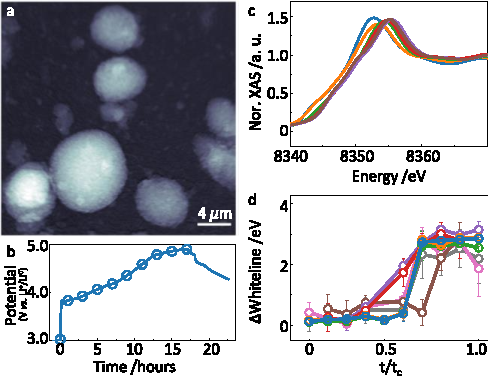
\includegraphics{figures/nca_txm.pdf}
  \caption{Operando \gls{txm} of \nca{} during first charge. (a) Mean
    optical depth frame of \nca{} particles. (b) Applied potential to
    operando cell during galvanostatic charging at
    \SI{0.05}{\ampere\per\ampere\per\hour} (C/20). (c) Normalized
    spectra from \emph{ex-situ} ensemble-average \gls{xas}. (d)
    State-of-charge determined by whiteline position relative to
    overall state of charge in (c) for individual particles of
    \nca{}. \textDelta{}whiteline is determined by the change in the
    energy of maximum absorbance of all pixels in a particle at a
    given time point relative to the energy of maximum absorbance for
    all particles in the pristine state. Error bars represent one
    standard deviation over pixels within the given particle. The
    horizontal axis in (d) shows the ratio of time since current was
    applied ($t$) to the total time to reach the cut-off potential
    ($t_c$).}
  \label{fig:txm-nca}
\end{figure}

\begin{figure}[!h]
  % beedrill/uic/operando-txm-graphics/Operando_Paper_Graphics.ipynb
  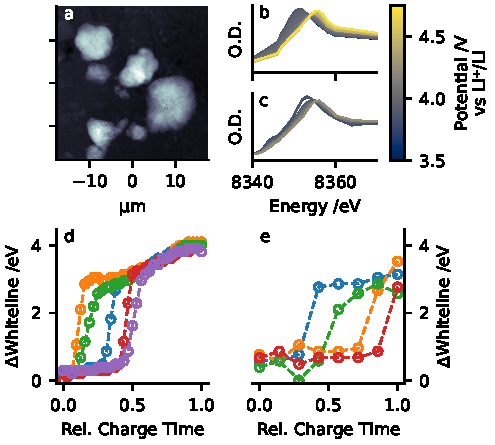
\includegraphics{figures/nmc_txm.pdf}
  \caption{Operando \gls{txm} \gls{xas} of \nmc[333]{} and \nmc[532]{}
    during first charge. (a) Mean optical depth frame of \nmc[333]{}
    particles. (b,c) Median optical depth spectra of active material
    during (b) second charge of \nmc[333]{} and (c) first charge of
    \nmc[532]{}. (d,e) Changes in median whiteline energies during
    first charge relative to start of charging for individual
    particles of (d) \nmc[333]{} (e) \nmc[532]{}. Arrows show
    correspondence between particles in (a) and lines in
    (d). \textDelta{}whiteline determination matches that described in
    Figure \ref{fig:txm-nca}.}
  \label{fig:txm-nmc}
\end{figure}

\newpage
\begin{figure}[!h]
  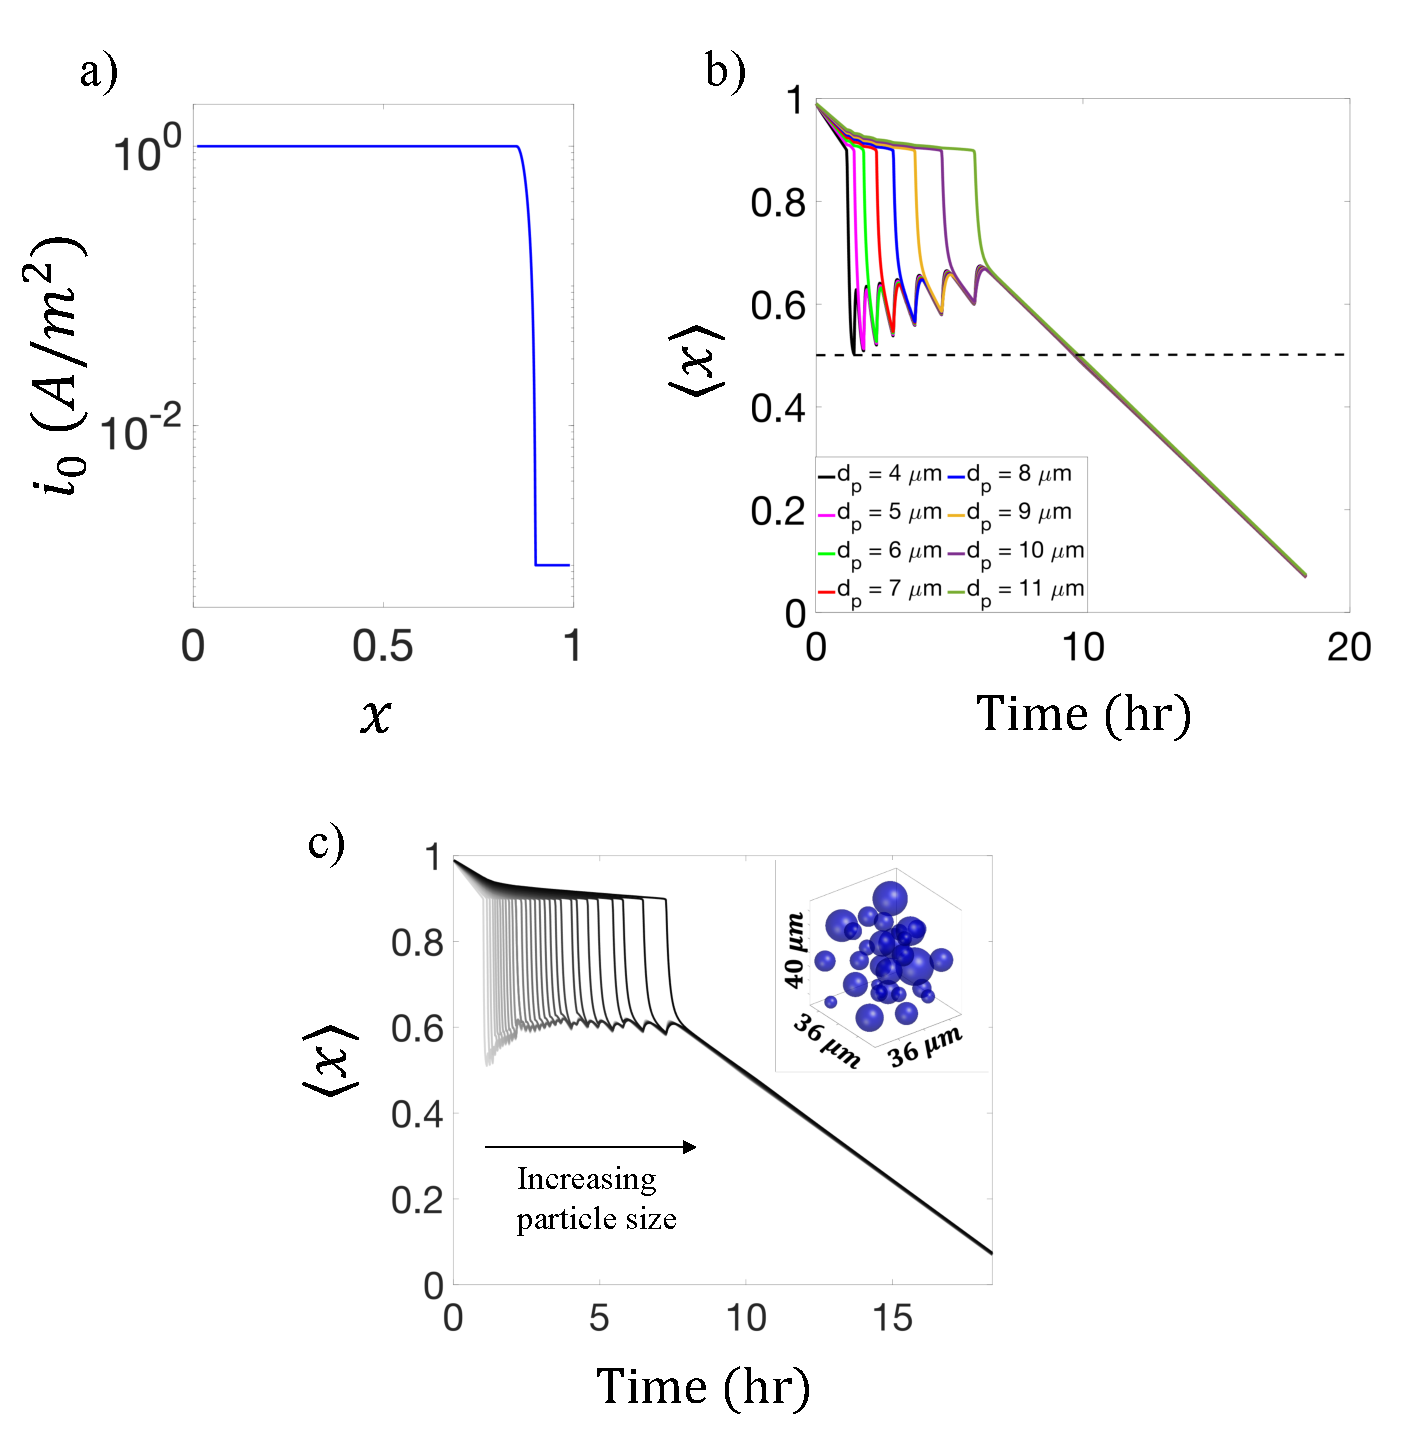
\includegraphics[scale =1]{figures/modeling_figure_1.pdf}
  \caption{(a) The model form of the \glsreset{ecd}\gls{ecd} vs.\ the
    local \glsreset{xLi}\gls{xLi} used for the simulation with a
    composition-dependent \gls{ecd}. (b) The simulated evolution of
    the volume-averaged Li-site fraction in individual particles,
    $\left\langle x_{\rm{Li}}\right\rangle $, for C/20 galvanostatic
    charging of the 8-particle system. (c) The simulated evolution of
    the volume-averaged Li-site fraction in individual particles,
    $\left\langle x_{\rm{Li}}\right\rangle $, for C/20 galvanostatic
    charging of the 30-particle system.}
  \label{fig:model-1}
\end{figure}

\newpage
\begin{figure}[!h]
  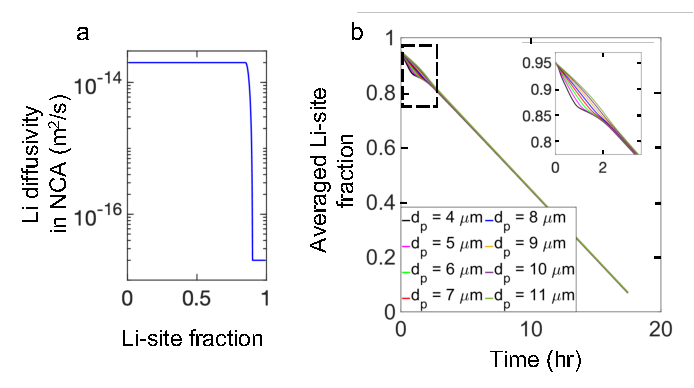
\includegraphics[scale =1]{figures/modeling_figure_2.pdf}
  \caption{(a) The model form of \gls{D_s} vs.\ the local
    \glsreset{xLi}\gls{xLi} used for the simulation with a
    composition-dependent diffusivity. Note that the form of the
    function is the same as that of \gls{ecd} shown above, including
    the ratio between the maximum and minimum values and the width of
    the transition. (b) The simulated evolution of the volume-averaged
    \gls{xLi} in individual particles, $\langle x_{\rm{Li}} \rangle$,
    for C/20 galvanostatic charging of the 8-particle system. The
    inset shows the magnified view of the section bounded by the
    dashed box.}
  \label{fig:model-2}
\end{figure}


\end{document}
